\chapter{Concluzii și direcții viitoare}
\label{chap:conclusions}

În această lucrare am prezentat problematica identificării defectelor într-o rețea de apă, prin analiza profilurilor reziduurilor într-o perioadă de timp corespunzătoare regimului staționar. Abordarea s-a axat pe alegerea unei metode empirice și statistice în detrimentul unei metode analitice, așa cum a fost prezentat și în capitolul \ref{chap:simulari}, o interpretare exactă a rețelelor de apă este foarte dificilă, procesul care stă în spatele dependenței presiune - debit - viteză în conducte fiind unul puternic neliniar și influențat de mulți factori exogeni. 

Abordarea propusă în această lucrare este una bine documentată \cite{irofti2017dictionary}, \cite{perelman2016sensor}, \cite{rossman2000epanet} asupra căreia am aplicat două metode de învățare automată supervizată - mașini cu vectori suport și învățarea de dicționare rare. De asemenea o preocupare a acestei lucrări a fost centrată asupra optimizării procesului de clasificare, anume reducerea numărului de senzori prezenți la clasificare. Motivația reducerii numărului de senzori este ajungerea la un compromis ingineresc între investiția în senzorii plasați în nodurile rețelei de apă și cheltuielile pentru combaterea defectelor. Rezultatul reducerii numărului de senzori prin metoda \eqref{alg:rfe} și prin rezolvarea problemei NP-Complete \eqref{eq:opt_problem}, a arătat prezența redundanței puternice între informațiile provenite de la senzori, în mod natural, deoarece nodurile vecine într-un graf sunt supuse unor solicitări foarte apropiate.

Rezultatele clasificării folosind metodele LC-DL și SVM au dat rezultate apreciabile și relevante din punct de vedere statistic, antrenarea și testarea fiind făcută pe două seturi de date echilibrate (i.e. același număr de obiecte pentru fiecare clasă) și variate - fiecare defect pentru care se încerca clasificarea avea ca exemple de clasă profiluri cu mai multe magnitudini - metricile de acuratețe atingând un procent foarte ridicat - 96.7\% pentru LC-DL folosind 10 senzori aleși cu MSC și 94.1\% pentru SVM folosind 10 senzori aleși cu RFE. De asemenea algoritmul SVM poate fi folosit într-un alt algoritm \ref{alg:rfe} pentru a putea alege nodurile din rețea cu cea mai importantă contribuție.

\begin{figure}[H]
\centering
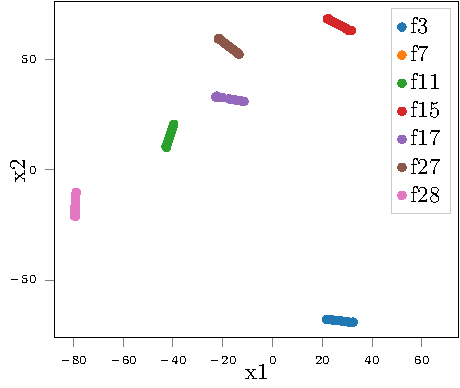
\includegraphics[width=0.45\textwidth]{\pics/c6_pics/2dfaults}
\caption{Proiecția în 2D a profilurilor defectelor}
\label{fig:tsne_faults}
\end{figure}

Ca ilustrație grafică bidimensională asupra profilurilor defectelor am realizat în figura \ref{fig:tsne_faults} proiecția pe 2 axe a vectorului de caracteristici al unui defect format din 31 de caracteristici, folosind algoritmul TSNE. După cum se poate observa aceste defecte nu numai ca sunt liniar separabile, dar în funcție de magnitudinea emițătorului în nodul respectiv proiecțiile $(x1, x2)$ se vor situa pe o dreaptă. Deși folosirea unei metode de clasificarea bazate pe extragerea proiecțiilor în 2D sau 3D prin algoritmul TSNE poate părea o idee atractivă, problema apare în momentul în care se dorește transformarea unui set de date nou - fiind un algoritm stocastic TSNE va da rezultate diferite la fiecare rulare și există riscul ca aceleași defecte să fie coagulate în alte zone ale planului bidimensional, compromițând astfel procesul de clasificare.


\paragraph{Direcții viitoare} \mbox{} \\

Ca abordare diferită putem să considerăm partiționarea rețelei în mai multe subgrafuri \cite{irofti2017dictionary}  cu scopul de a relaxa problema și de a crește performanțele clasificării. O modalitate de a vedea care sunt nodurile care oferă cea mai mare apropiere în sensul partiționării este folosirea unui algoritm de clusterizare asupra reziduurilor fiecărui defect, de exemplu K-Means \cite{k-means}. Rularea acestui algoritm cu 5 centroide dă următoarea cofigurație de clustere:

\begin{itemize}
    \item $C_1 = \{22, 23, 24, 27, 28, 29, 30, 31\}$
    \item $C_2 = \{1, 2, 3, 16, 17, 18, 19\}$
    \item $C_3 = \{  20, 21\}$
    \item $C_4 = \{ 4, 5, 6, 7, 8, 9, 10, 11, 12, 13\}$
    \item $C_5 = \{ 25, 26, 14, 15\}$
\end{itemize}

Rulând algoritmul de clasificare de la capitolul \ref{chap:ml_classification} obținem o acuratețe de 95.2\% cu ajutorul a suportului de 4 senzori selectați $C=\{12, 19, 25, 27\}$
% [{22, 23, 24, 27, 28, 29, 30, 31}, {1, 2, 3, 16, 17, 18, 19}, {20, 21}, {4, 5, 6, 7, 8, 9, 10, 11, 12, 13}, {25, 26, 14, 15}]


